\chapter{Écrans de l'interface}
\label{annexe:ecrans}

Cette annexe présente les écrans concrets de l'interface décrite à la section~\ref{sec:soft_ui}, ainsi que la barre de statut et l'écran de veille dont le corps ne donnait qu'une description sommaire. Les captures sont prises à la résolution native de 176 sur 176 pixels, ce qui rend visible le style pixel par pixel voulu pour l'interface.

Une barre de statut occupe la bande supérieure de tous les écrans qui suivent. Elle réunit trois indications, de gauche à droite l'état de la radio Bluetooth sous forme d'une antenne dont la couleur et les ondes distinguent la radio éteinte, allumée et liée, la sortie audio active au centre avec un libellé blanc pour la prise casque et bleu pour le Bluetooth, et le niveau de charge à droite passant au rouge à l'approche du seuil critique. Aucun trait ne souligne cette barre. Un segment horizontal occupant toute la largeur allumerait en effet des pixels sur une ligne entière de cette dalle passive, dont le courant appelé creuserait la tension du rail commun et ternirait la ligne, raison pour laquelle le menu d'accueil délimite lui aussi ses sélections par des crochets d'angle plutôt que par un cadre plein.

\begin{figure}[H]
    \centering
    \begin{subfigure}[t]{0.30\textwidth}\centering
        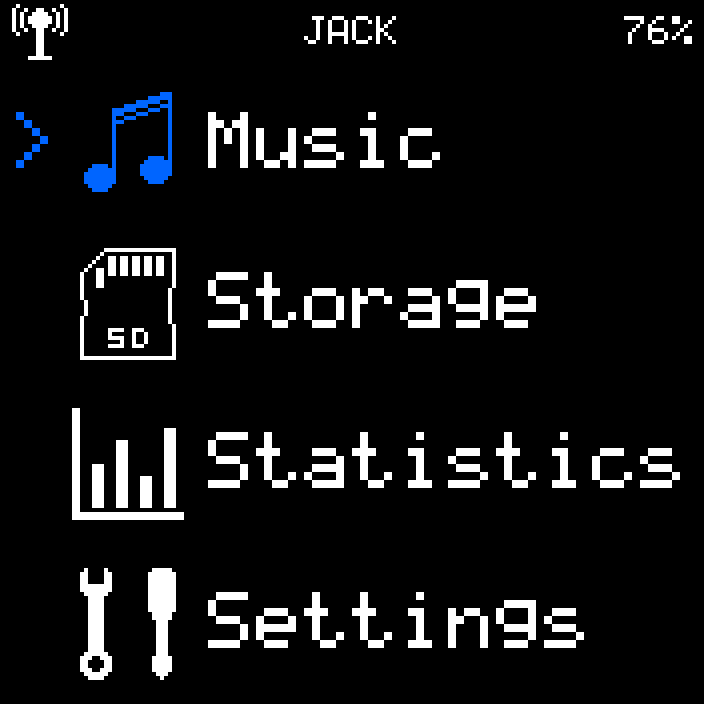
\includegraphics[width=\linewidth]{assets/figures/root_menu.png}
        \caption{Menu d'accueil}
    \end{subfigure}\hfill
    \begin{subfigure}[t]{0.30\textwidth}\centering
        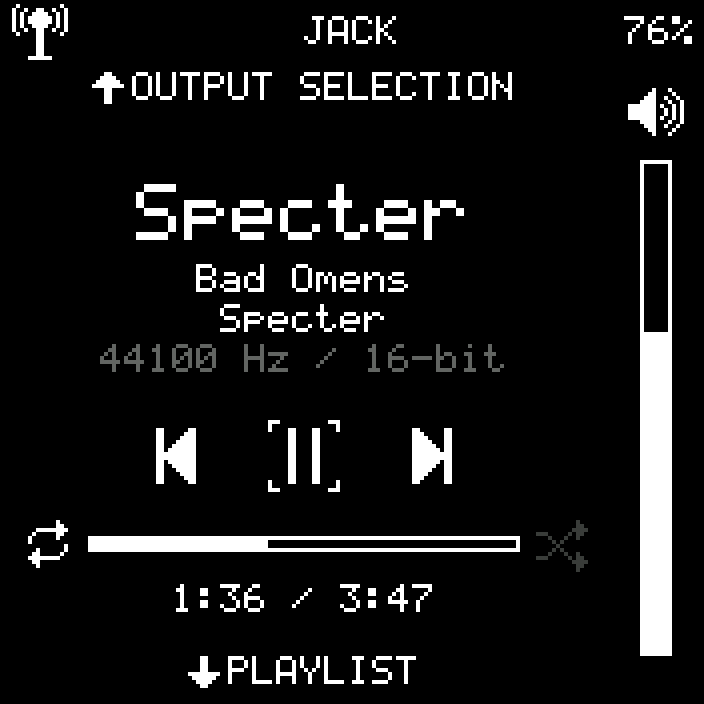
\includegraphics[width=\linewidth]{assets/figures/now_playing.png}
        \caption{Lecture en cours}
    \end{subfigure}\hfill
    \begin{subfigure}[t]{0.30\textwidth}\centering
        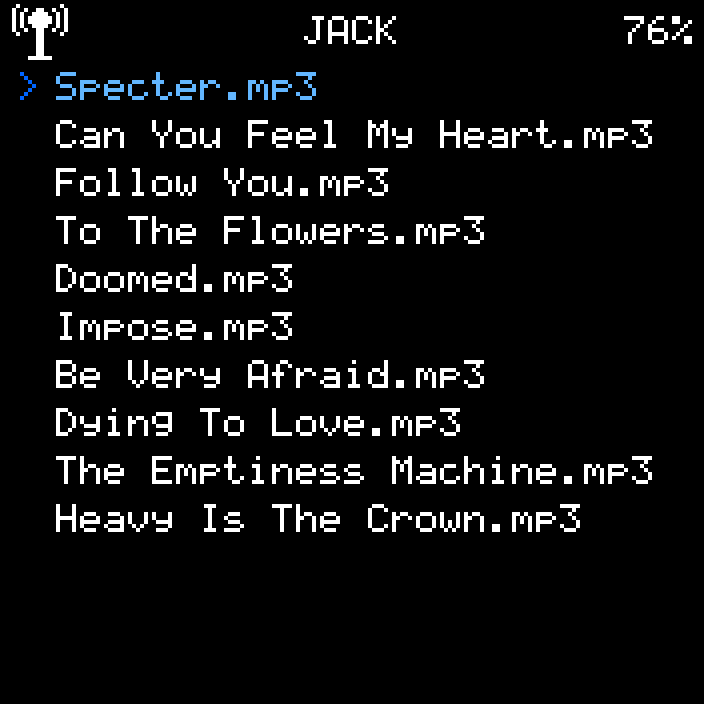
\includegraphics[width=\linewidth]{assets/figures/playlist_browser.png}
        \caption{Navigateur de pistes}
    \end{subfigure}

    \vspace{4mm}
    \begin{subfigure}[t]{0.30\textwidth}\centering
        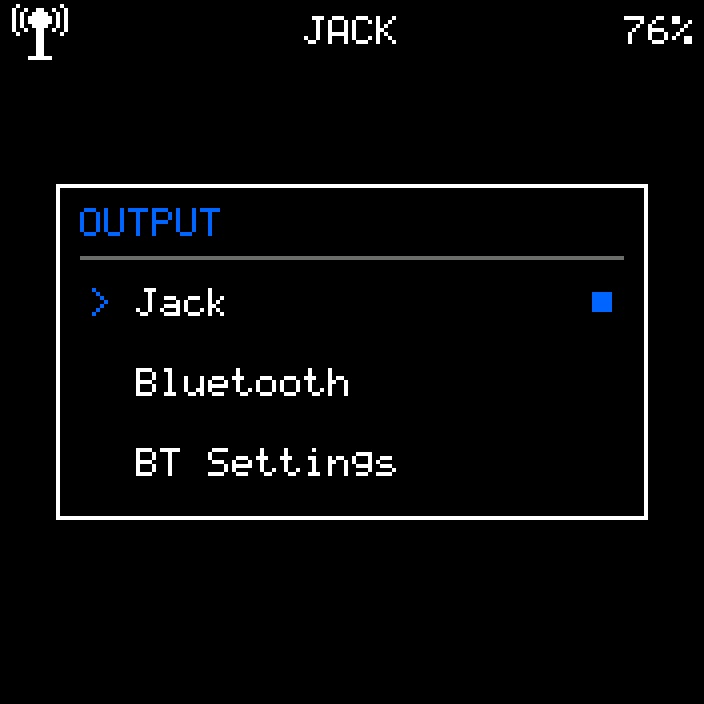
\includegraphics[width=\linewidth]{assets/figures/output_select.png}
        \caption{Sélection de la sortie audio}
    \end{subfigure}
    \caption{Écrans de lecture et de navigation principale.}
    \label{fig:ecrans-lecture}
\end{figure}

\begin{figure}[H]
    \centering
    \begin{subfigure}[t]{0.30\textwidth}\centering
        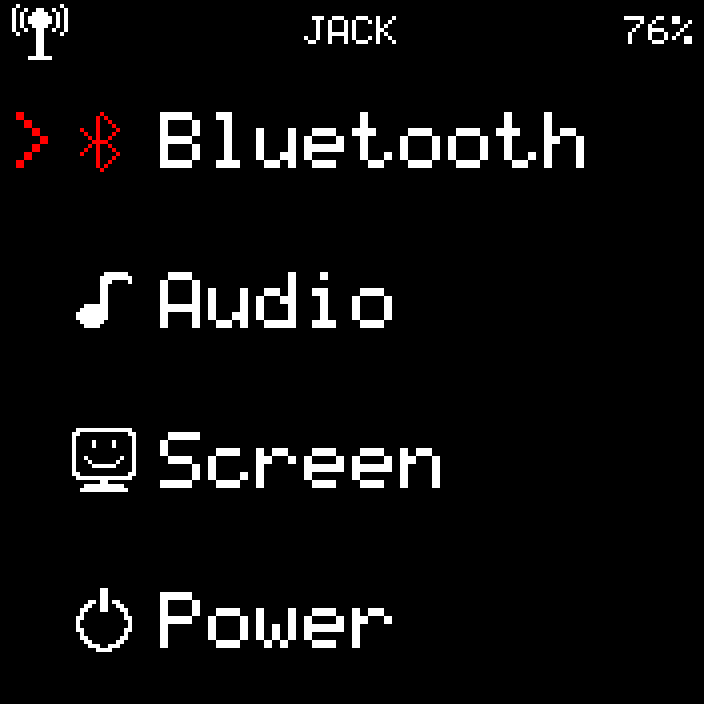
\includegraphics[width=\linewidth]{assets/figures/settings_menu.png}
        \caption{Menu des réglages}
    \end{subfigure}\hfill
    \begin{subfigure}[t]{0.30\textwidth}\centering
        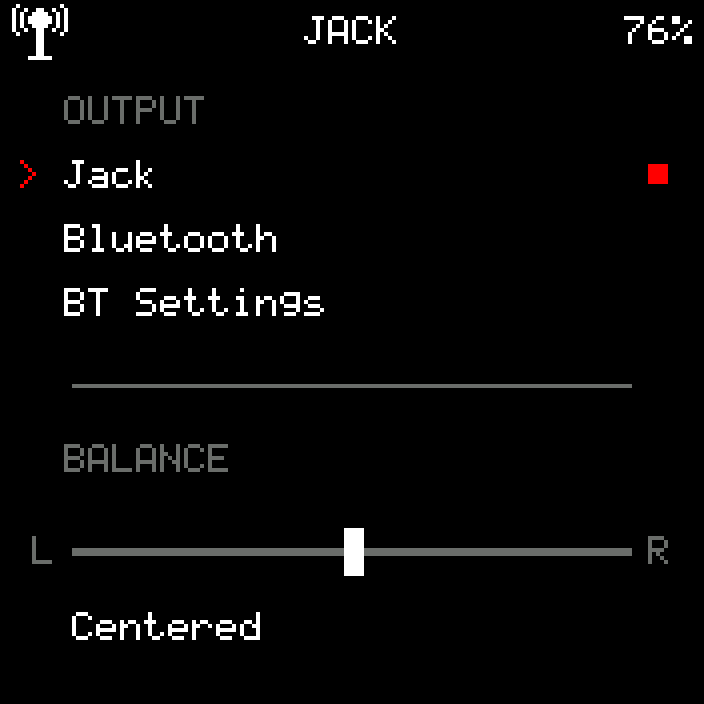
\includegraphics[width=\linewidth]{assets/figures/audio_settings.png}
        \caption{Réglages audio}
    \end{subfigure}\hfill
    \begin{subfigure}[t]{0.30\textwidth}\centering
        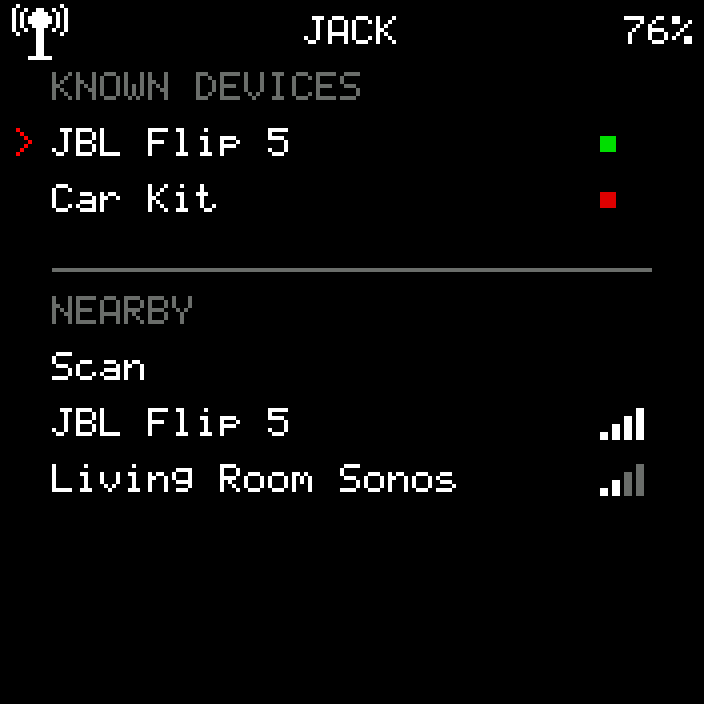
\includegraphics[width=\linewidth]{assets/figures/bluetooth_settings.png}
        \caption{Réglages Bluetooth}
    \end{subfigure}

    \vspace{4mm}
    \begin{subfigure}[t]{0.30\textwidth}\centering
        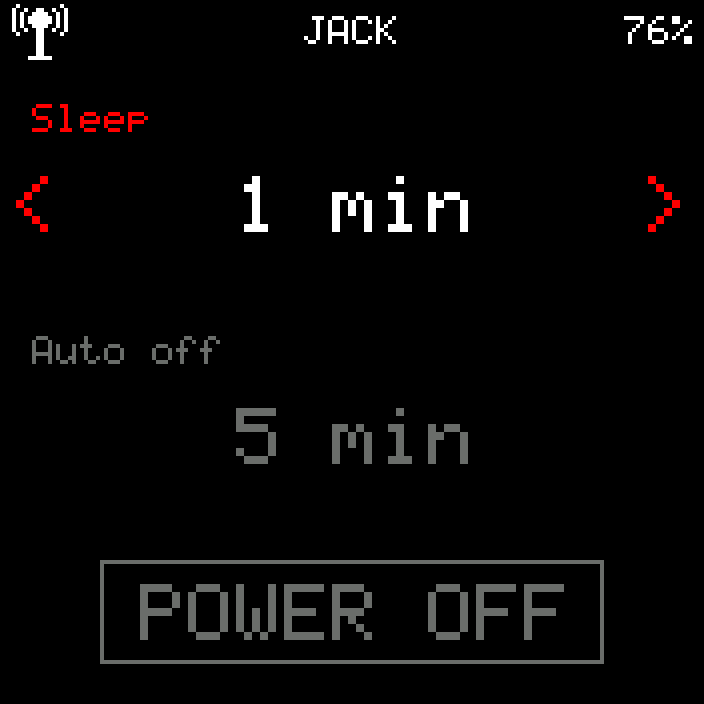
\includegraphics[width=\linewidth]{assets/figures/power_settings.png}
        \caption{Réglages d'alimentation}
    \end{subfigure}\hfill
    \begin{subfigure}[t]{0.30\textwidth}\centering
        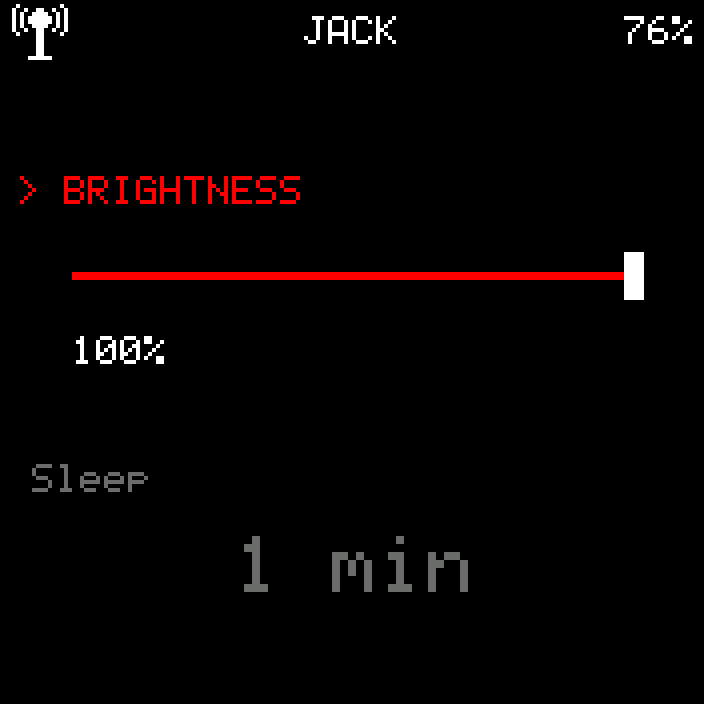
\includegraphics[width=\linewidth]{assets/figures/screen_settings.png}
        \caption{Réglages de l'écran}
    \end{subfigure}
    \caption{Écrans de réglages.}
    \label{fig:ecrans-reglages}
\end{figure}

\begin{figure}[H]
    \centering
    \begin{subfigure}[t]{0.30\textwidth}\centering
        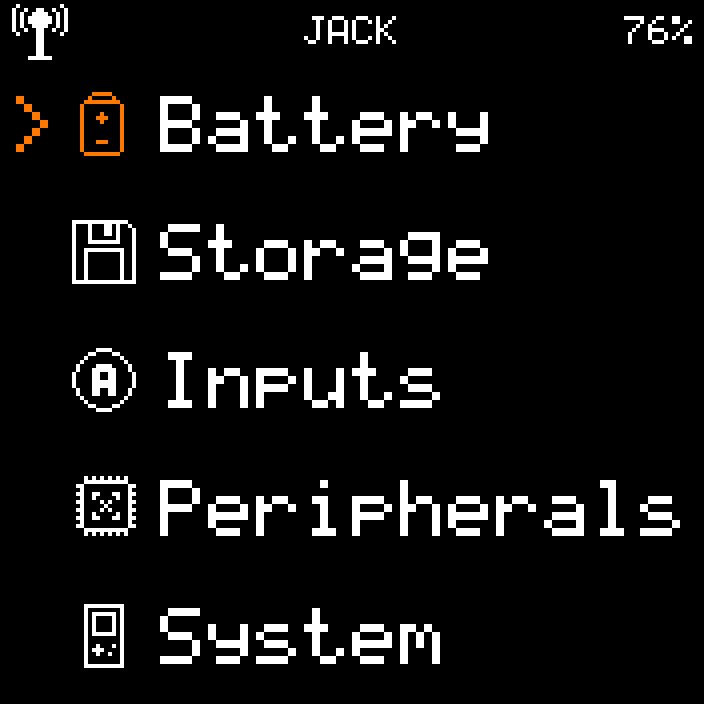
\includegraphics[width=\linewidth]{assets/figures/stats_menu.png}
        \caption{Menu des statistiques}
    \end{subfigure}\hfill
    \begin{subfigure}[t]{0.30\textwidth}\centering
        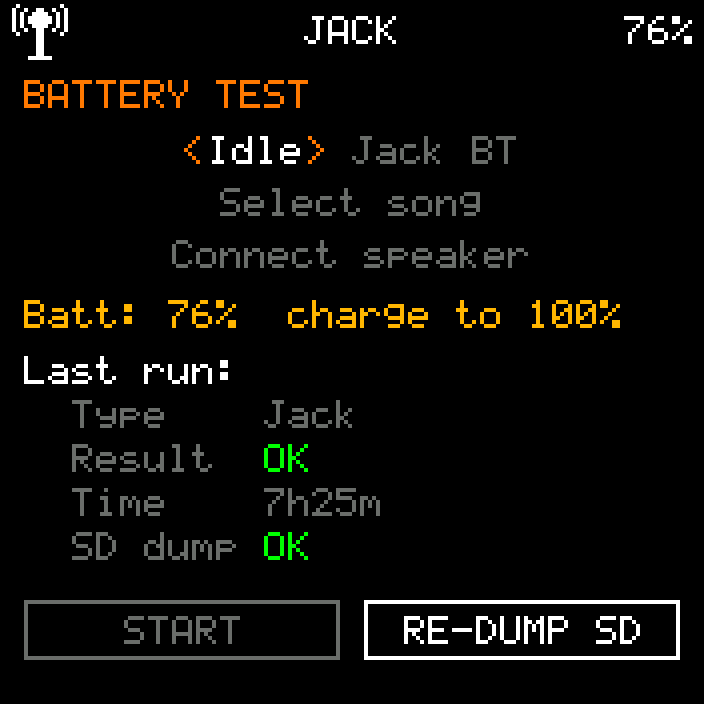
\includegraphics[width=\linewidth]{assets/figures/battery_test.png}
        \caption{Test d'autonomie}
    \end{subfigure}\hfill
    \begin{subfigure}[t]{0.30\textwidth}\centering
        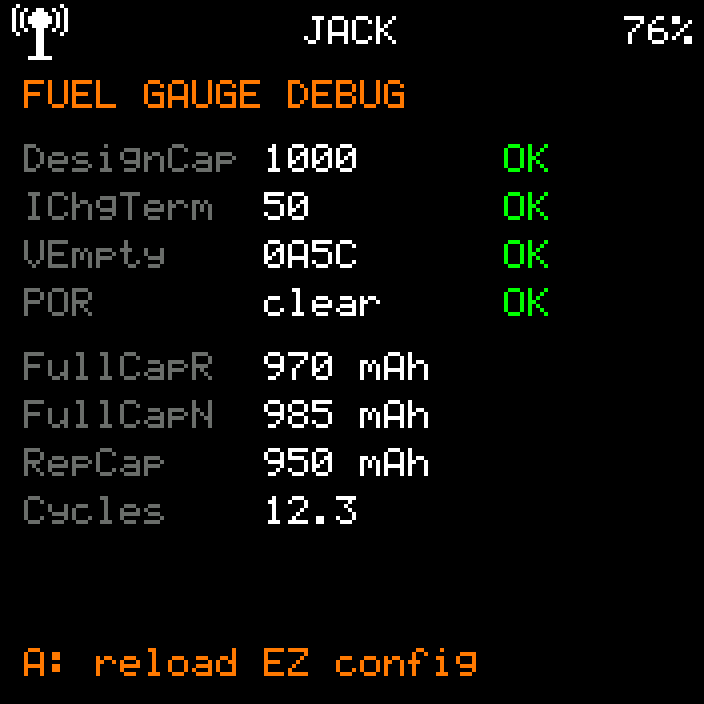
\includegraphics[width=\linewidth]{assets/figures/fuel_gauge_debug.png}
        \caption{Diagnostic de la jauge de charge}
    \end{subfigure}

    \vspace{4mm}
    \begin{subfigure}[t]{0.30\textwidth}\centering
        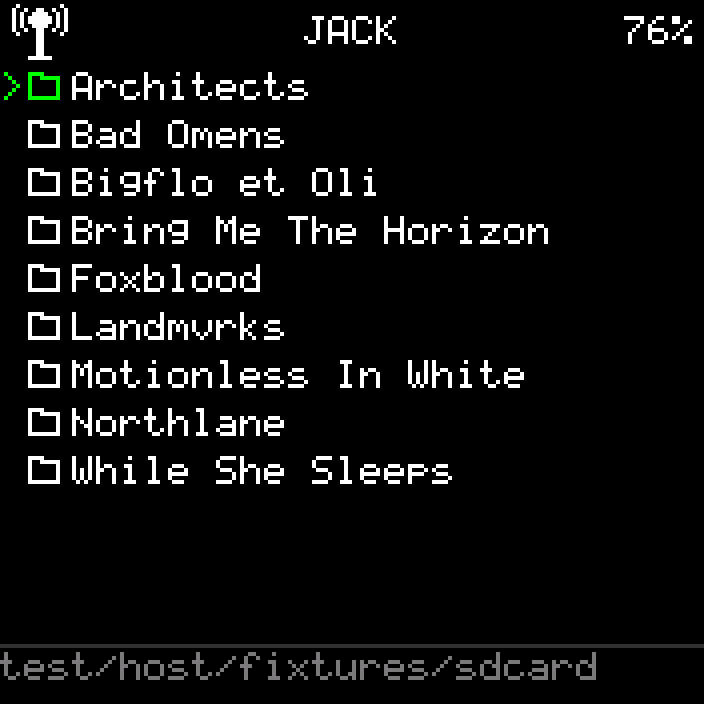
\includegraphics[width=\linewidth]{assets/figures/storage_screen.png}
        \caption{État du stockage}
    \end{subfigure}
    \caption{Écrans de statistiques et de diagnostic.}
    \label{fig:ecrans-diag}
\end{figure}

L'écran de veille, évoqué à la section~\ref{sec:ui_verrouillage}, ne figure pas dans la galerie car il ne s'agit pas d'un écran de navigation. Il se réduit à une trame noire portant les mots « Sleep mode » et « Press A to wake up » en gris sombre, la lettre du bouton de réveil étant cerclée à l'image du bouton physique. Le tracé du cercle emploie l'algorithme du point milieu, sans bibliothèque. Pendant toute la durée du verrouillage, ce texte est redessiné toutes les trente secondes à l'une de cinq positions légèrement décalées, parcourues cycliquement, afin qu'aucun pixel allumé ne demeure au même endroit assez longtemps pour marquer la dalle. Le coût d'un tel redessin, un rendu de trame et un envoi, reste négligeable au regard de son espacement.